\documentclass[pdflatex,compress,mathserif]{beamer}

%\usetheme[dark,framenumber,totalframenumber]{ElektroITK}
\usetheme[darktitle,framenumber,totalframenumber]{ElektroITK}
\usepackage[utf8]{inputenc}
\usepackage[T1]{fontenc}
\usepackage{lmodern}
\usepackage{amsmath}
\usepackage{amsfonts}
\usepackage{amssymb}
\usepackage{graphicx}
\usepackage{multicol}
\usepackage{lipsum}
\setbeamertemplate{caption}[numbered]\setbeamertemplate{caption}[numbered]
\newcommand*{\Scale}[2][4]{\scalebox{#1}{$#2$}}%

\title{Signals and Systems}
\subtitle{Laplace Transform}

\author{Mifta Nur Farid}

\begin{document}

\maketitle

\begin{frame}
	\frametitle{Introduction}
	\begin{figure}
		\centering
		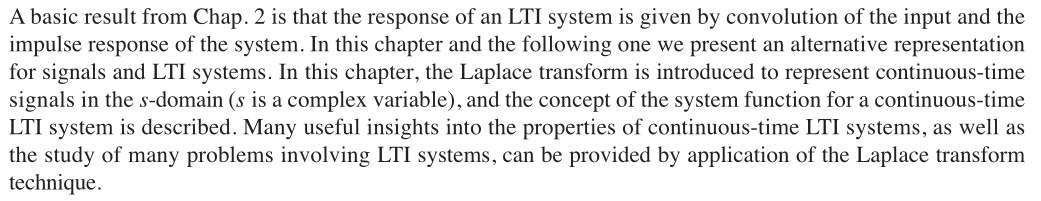
\includegraphics[width=\linewidth]{img/img01}
	\end{figure}
\end{frame}

\begin{frame}
	\frametitle{The Laplace Transform}
	\begin{figure}
		\centering
		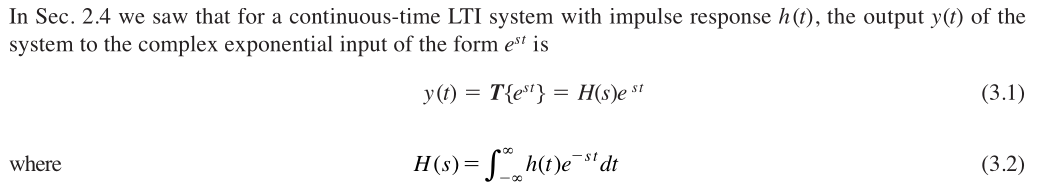
\includegraphics[width=\linewidth]{img/img02}
	\end{figure}
\end{frame}

\begin{frame}
	\frametitle{Definition}
	\begin{figure}
		\centering
		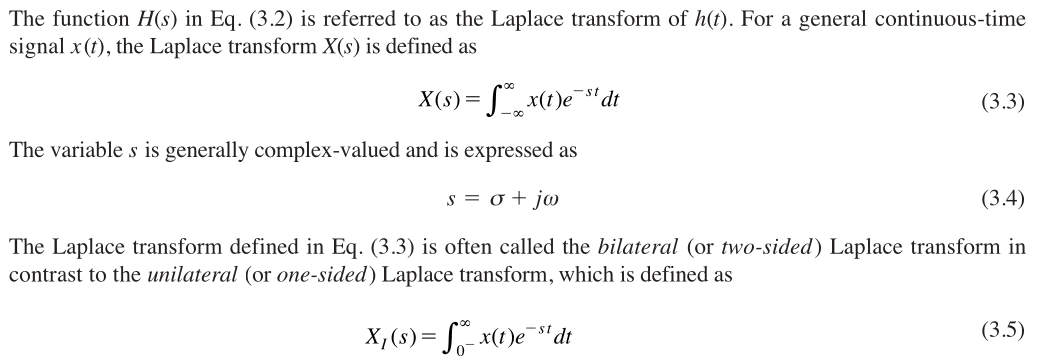
\includegraphics[width=\linewidth]{img/img03}
	\end{figure}
\end{frame}

\begin{frame}{Definition}
	\begin{figure}
		\centering
		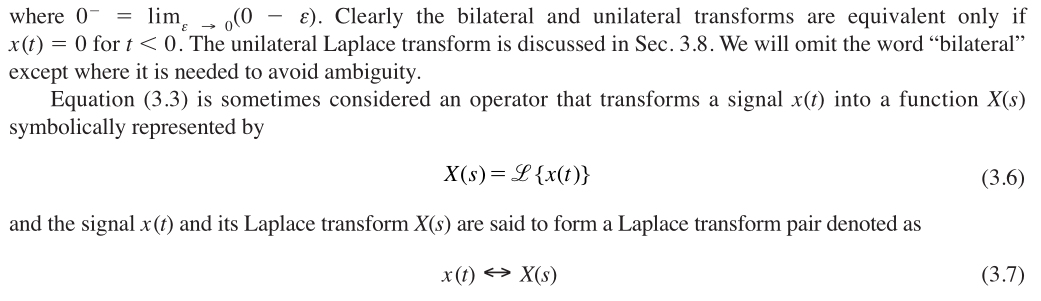
\includegraphics[width=\linewidth]{img/img04}
	\end{figure}
\end{frame}

\begin{frame}
	\frametitle{The Region of Convergence}
	\begin{figure}
		\centering
		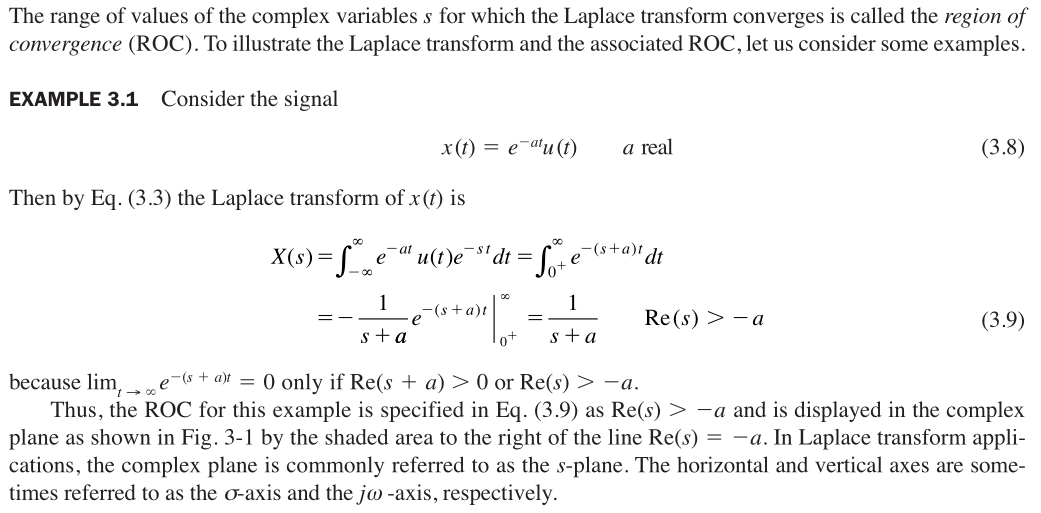
\includegraphics[width=\linewidth]{img/img05}
	\end{figure}
\end{frame}

\begin{frame}{The Region of Convergence}
	\begin{figure}
		\centering
		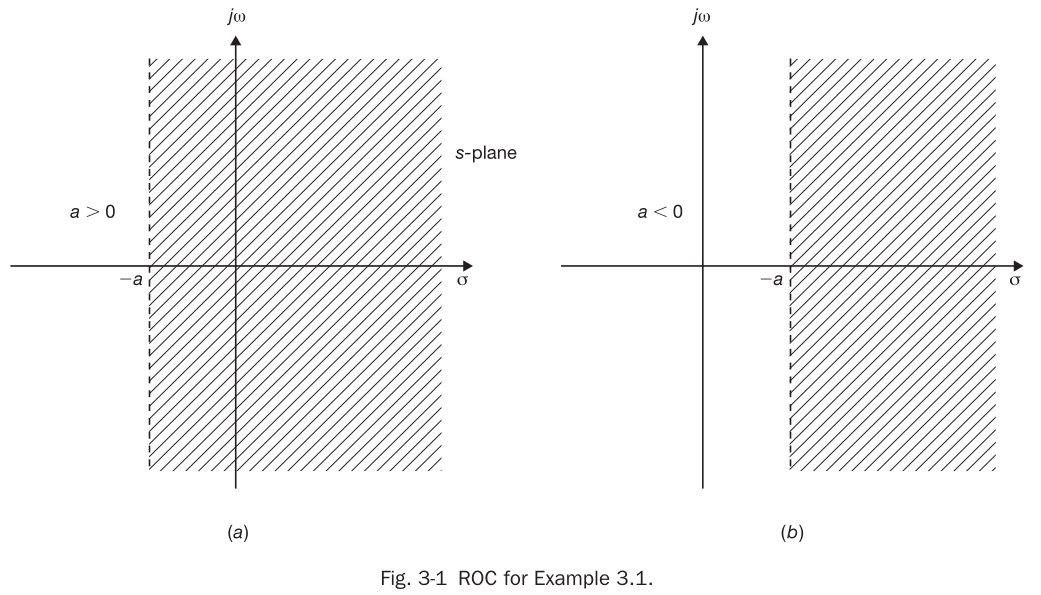
\includegraphics[width=\linewidth]{img/img06}
	\end{figure}
\end{frame}

\begin{frame}{The Region of Convergence}
	\begin{figure}
		\centering
		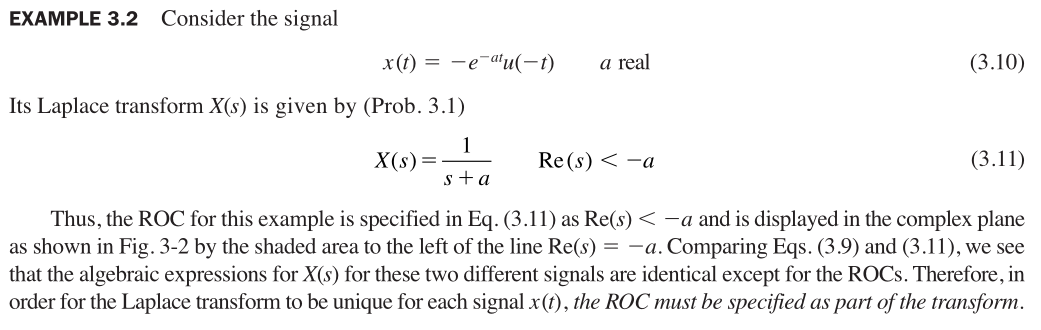
\includegraphics[width=\linewidth]{img/img07}
	\end{figure}
\end{frame}

\begin{frame}{The Region of Convergence}
	\begin{figure}
		\centering
		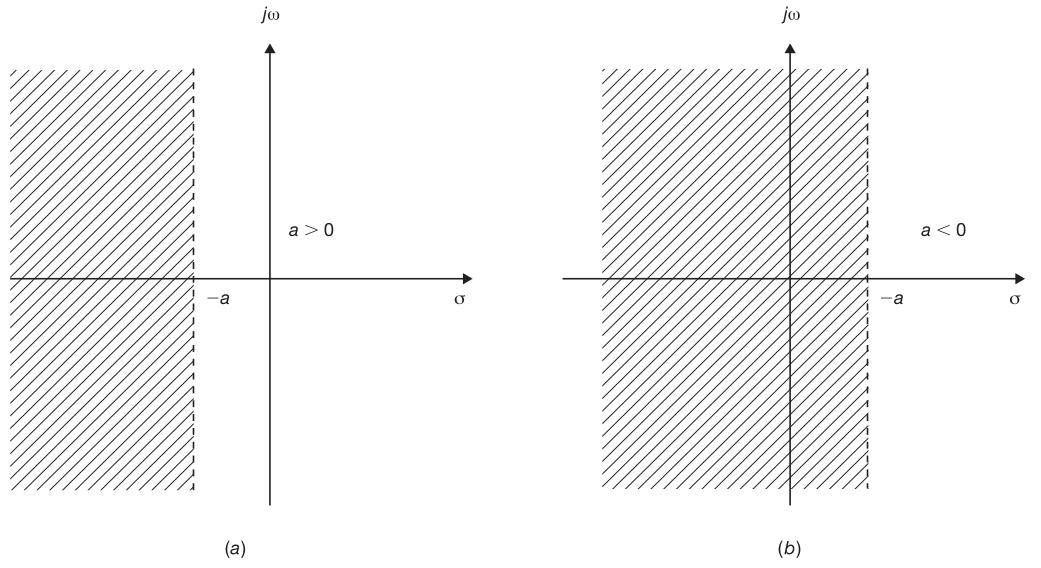
\includegraphics[width=\linewidth]{img/img08}
	\end{figure}
\end{frame}

\begin{frame}
	\frametitle{Poles and Zeros of X(s)}
	\begin{figure}
		\centering
		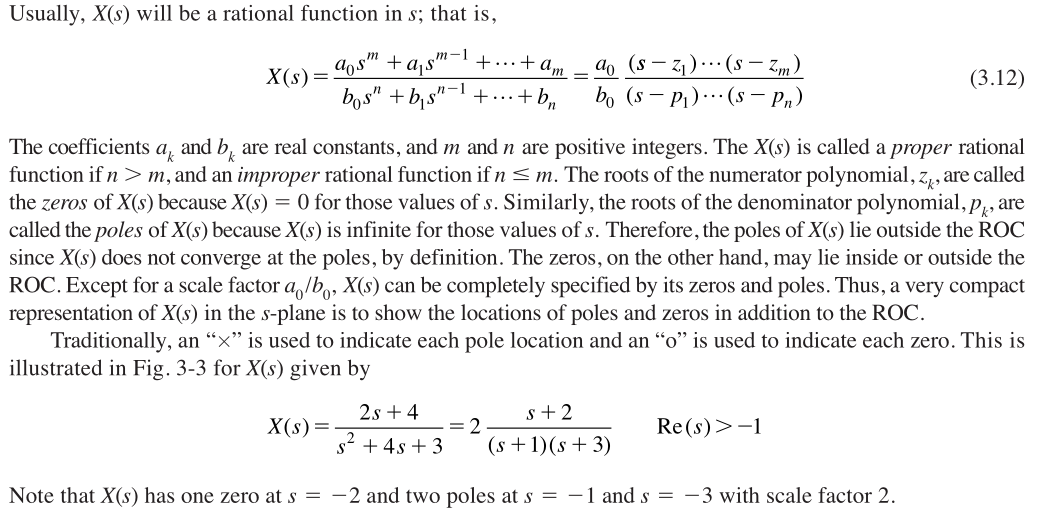
\includegraphics[width=\linewidth]{img/img09}
	\end{figure}
\end{frame}

\begin{frame}{Poles and Zeros of X(s)}
	\begin{figure}
		\centering
		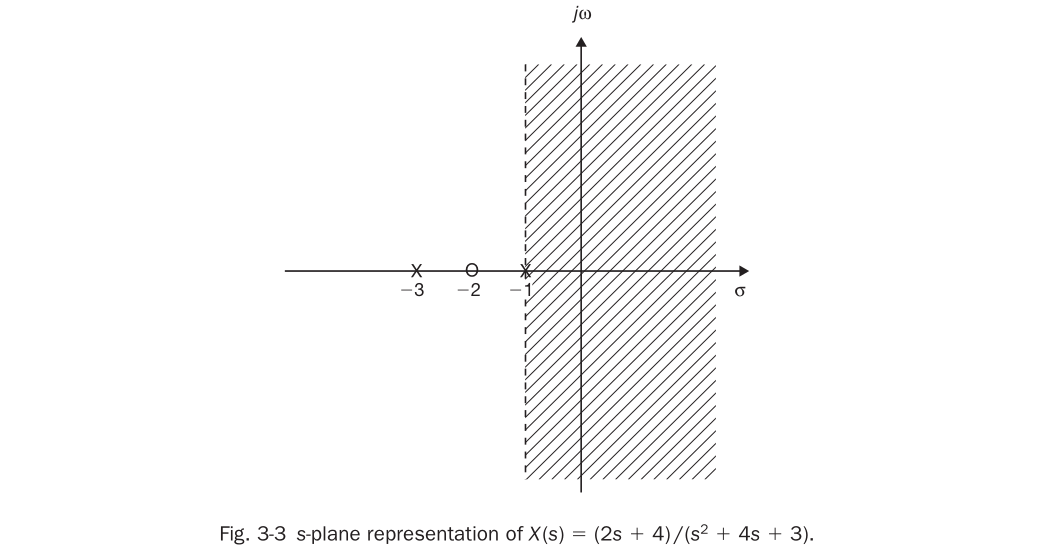
\includegraphics[width=\linewidth]{img/img10}
	\end{figure}
\end{frame}

\end{document}
